\documentclass[a4paper,12pt]{article}
\usepackage[margin=2cm]{geometry}

\usepackage{comment}
\usepackage{longtable}
\usepackage{tabularx,booktabs}
\usepackage{listings}
\usepackage{graphicx}

\lstset{basicstyle=\ttfamily}
\newcommand{\py}{\lstinline}

% Math notations
\newcommand{\Z}{{\mathbb{Z}}}                     % set of integers
\usepackage{amsmath,amssymb,wasysym}

% MoA notations
\newcommand{\minus}{{}^{\boldsymbol{\mbox{-}}\!}} % scalar negation operator
\newcommand{\rop}[1]{\,\mathrm{#1}^*\,}           % relational operation
\newcommand{\op}[1]{\,\mathrm{#1}\,}              % binary operation
\newcommand{\uop}[1]{\mathrm{#1}\,}               % unary operation
\newcommand{\hop}[2]{{{}_{#1}\!\Omega_{#2}}\,}      % higher order operation
\newcommand{\id}[1]{\mathrm{id}(\op{#1})}         % identity of operations
\newcommand{\dims}{\delta\,}                      % array dimension operator
\newcommand{\shape}{\rho\,}                       % array shape operator
\newcommand{\size}{\tau\,}                        % array size operator
\newcommand{\reshape}{\,\widehat{\rho}\,}         % reshape operator
\newcommand{\drop}{\,\nabla\,}                    % drop operator
\newcommand{\take}{\,\Delta\,}                    % take operator
\newcommand{\product}{\pi\,}                      % product operator
\DeclareMathOperator{\rav}{rav}
\newcommand{\ravel}{\rav\,}                       % ravel operator
\newcommand{\range}{\iota\,}                      % range operator
\newcommand{\transpose}{\bigcirc\!\!\!\!\!\backslash\;} % transpose operator, need a better symbol
\newcommand{\vc}[1]{<#1>}                         % vector with one component
\newcommand{\vcc}[2]{<#1\;#2>}                    % vector with two components
\newcommand{\vccc}[3]{<#1\;#2\;#3>}               % vector with four components
\newcommand{\outerprod}[1]{\,\bullet_{#1}\,}              % outer product opetation
\newcommand{\innerprod}[2]{\,{}_{#1}\!\!\bullet_{#2}\,}   % inner product opetation
\DeclareMathOperator{\red}{red}
\newcommand{\reduce}[1]{{}_{#1}\!\red\,}          % reduce operator
\newcommand{\getitem}[2]{{#2}\,\psi\,{#1}}        % psi operator


\newcommand{\scan}[1]{{}_{\op{#1}\!}\mathrm{scan}\,}
\newcommand{\kron}{\bigcirc\,\!\!\!\!\!\!\times\;}
\newcommand{\cat}{+\!\!\!+}
\newcommand{\gu}{\mathrm{gu}\,}
\newcommand{\gd}{\mathrm{gd}\,}
\newcommand{\compress}{\,\notslash\,}
\newcommand{\expand}{\,\notbackslash\,}
\newcommand{\reverse}{\phi\,}
\newcommand{\rotate}[1]{{#1}\theta\,}


\title{MoA formalism and arrays in software}
\author{Pearu Peterson and Hameer and Saul and Lenore and Travis\\
Quansight, Labs}

\begin{document}
\maketitle
\section{Introduction}

MoA - Mathematics of Arrays - defines a formalism (based on APL) to
describe multidimensional arrays and operations on these. On the other
hand, contemporary array processing software (NumPy, Xnd, Apache
Arrow, etc) implement multidimensional array container objects and
define UI to interact with the array objects. The aim of this document
is to provide a mapping between MoA formalism and UI-s of widely used
array processing software.

\section{Basic definitions}

The MoA formalism is originally defined in ``A Mathematics of Arrays''
by Lenore Mullin, PhD thesis, 1988\cite{mul00}.  We use NumPy
\cite{travis0} user interface as a representative of a software
implementing UI for multidimensional arrays. For brevity, we assume
\verb+from numpy import *+.

\noindent
In general, \emph{an array is an object that has a mapping to get
  array items} \footnote{A mapping $f$ is a set of argument and value
  pairs,$(i,v)$, and is represented as $f(i)=v$. We consider only
  single-valued mappings.} . The arguments to the mapping are called
\emph{indices}, all valid indices define the so-called \emph{index
  set} of an array. The items can be arbitrary objects.
Two arrays are \emph{equal} iff their get items mappings are equal: their shapes and components are equivalent.
\emph{Element-wise operations} of two arrays are defined iff the index
sets of the two arrays are equal.
Arrays can be classified according to how the mappings are defined:
\begin{description}
\item[Multidimensional arrays:] The index set of
  an $N$-dimensional array is an $N$-dimensional hyperrectangle in
  $\Z^N$: $[0,\ldots,s_0-1]\times\cdots\times[0,\ldots,s_{N-1}-1]$
  where non-negative integers $(s_0,\ldots,s_{N-1})$ define the shape
  of an array.
\item[Ragged arrays:] The index set of an
  $N$-dimensional ragged array is a connected subset of an
  $N$-dimensional hyperrectangle in $\Z^N$. The concrete
  representation of the index set may have different forms.
\item[Sparse arrays:] The index set of an sparse array is a possibly
  disconnected subset of $N$-dimensional hyperrectangle in $\Z^N$ and
  is extended to the full hyperrectangle by defining the default
  value.
\end{description}

The MoA deals with multidimensional arrays only.  The NumPy implements
array object for multidimensional arrays only. There is one-to-one
relation between MoA formalism and NumPy UI.

\section{Optimization of Arrays in NumPy: Dense to Start}
We show how the inclusion of MoA and the Psi Calculus for dense arrays
reduces to a normal form. This is a powerful concept in that programmers may design an algorithm differently, one may be efficient, another may not, even if the answer is the same. 
\noindent
We show that there will not be performance issues for that choice because all algorithms using the MoA algebra will reduce to the same normal form. Another important concept is that all intermediate arrays are eliminated. Performance analysis and graphs will show this.

\subsection{An example}

In the following we demonstrate how to reduce a NumPy array expression
to its normal form using MoA.

Consider the following NumPy arrays
\begin{verbatim}
>>> A = np.arange(30).reshape((2,3,5))
>>> B = 2 + A
>>> A
array([[[ 0,  1,  2,  3,  4],
        [ 5,  6,  7,  8,  9],
        [10, 11, 12, 13, 14]],

       [[15, 16, 17, 18, 19],
        [20, 21, 22, 23, 24],
        [25, 26, 27, 28, 29]]])
>>> B
array([[[ 2,  3,  4,  5,  6],
        [ 7,  8,  9, 10, 11],
        [12, 13, 14, 15, 16]],

       [[17, 18, 19, 20, 21],
        [22, 23, 24, 25, 26],
        [27, 28, 29, 30, 31]]])
\end{verbatim}
that in MoA formalism are represented as
\begin{align}
  A^3 &\equiv \vccc235\reshape(\range30), \\
  B^3 &\equiv 2+A^3,
\end{align}
and the following array expression as an example case
\begin{verbatim}
>>> r = np.inner(A[1,0,:], np.outer(A[1,0,:], B[0,1,:])[2,:])
>>> r
13175
\end{verbatim}
that in MoA formalism reads
\begin{equation}
r \equiv (\vcc10\psi A^3) \innerprod+\times (\vc2\psi((\vcc10\psi A^3) \outerprod\times (\vcc01\psi B^3))).
\end{equation}
Note that when evaluating the array expression directly, the
computation involves 30 multiplication and 4 addition
operations. Using MoA, we reduce the above array expression to its
normal form where the number of operations is minimal.

First, the items of the left operand of the inner product are
\begin{align*}
  \getitem{(\vcc10\psi A^3)}{\vc i} = \getitem{A^3}{\vccc10i}
\end{align*}
The items of the right operand of the inner product are
\begin{align}
&\getitem{
  (\getitem{((\getitem{A^3}{\vcc10}) \outerprod\times (\getitem{B^3}{\vcc01}))}{\vc2})
}{\vc i} \\
&\equiv \getitem{((\getitem{A^3}{\vcc10}) \outerprod\times (\getitem{B^3}{\vcc01})))}{\vcc2i} \\
&\equiv \getitem{(\getitem{A^3}{\vcc10})}{\vc2} \times \getitem{(\getitem{B^3}{\vcc01})}{\vc i}\\
&\equiv \getitem{A^3}{\vccc102} \times \getitem{B^3}{\vccc01i}
\end{align}
As a result, we have
\begin{align*}
  r &\equiv ((\vcc10\psi A^3) \innerprod+\times  \getitem{B^3}{\vcc01})\times\getitem{A^3}{\vccc102}
\end{align*}
that in NumPy syntax reads
\begin{verbatim}
>>> r_nf = np.inner(A[1,0,:], B[0,1,:]) * A[1,0,2]
\end{verbatim}
which contains 6 multiplications and 4 additions.

\subsection{A Small Example (TO BE REMOVED)}
Let's look at two NumPy expresssions. we  use small shapes to help the reader go through an expression to validate results. Large sizes are used in experiments to demonstrate conjectures. 
\begin{verbatim}   
>>> a=np.arange(30).reshape((2,3,5))
>>> a
array([[[ 0,  1,  2,  3,  4],
        [ 5,  6,  7,  8,  9],
        [10, 11, 12, 13, 14]],

       [[15, 16, 17, 18, 19],
        [20, 21, 22, 23, 24],
        [25, 26, 27, 28, 29]]])
        >>> b=a+2
>>> b
array([[[ 2,  3,  4,  5,  6],
        [ 7,  8,  9, 10, 11],
        [12, 13, 14, 15, 16]],

       [[17, 18, 19, 20, 21],
        [22, 23, 24, 25, 26],
        [27, 28, 29, 30, 31]]])
        >>> a.shape
(2, 3, 5)
>>> a[:,0,:]
array([[ 0,  1,  2,  3,  4],
       [15, 16, 17, 18, 19]])
>>> a[:,0,:][1,]
array([15, 16, 17, 18, 19])
>>> 
>>> 
>>> A=a[:,0,:][1,]
>>> B=b[:,1,:][0,]
>>> np.multiply.outer(A,B)
array([[105, 120, 135, 150, 165],
       [112, 128, 144, 160, 176],
       [119, 136, 153, 170, 187],
       [126, 144, 162, 180, 198],
       [133, 152, 171, 190, 209]])
>>> C=np.multiply.outer(A,B)
>>> A
array([15, 16, 17, 18, 19])
>>> B
array([ 7,  8,  9, 10, 11])
>>> C
array([[105, 120, 135, 150, 165],
       [112, 128, 144, 160, 176],
       [119, 136, 153, 170, 187],
       [126, 144, 162, 180, 198],
       [133, 152, 171, 190, 209]])
>>> C[2,:]
array([119, 136, 153, 170, 187])
>>> A * C[2,:]
>>> np.inner(A,C[2,:])
13175
\end{verbatim}
     
Let's reduce an expression to
a Denotational Normal Form (DNF), a semantic normal form that is not yet aware of memory layout or architectural components: vector registers, DMAs, etc.
We put all the expressions above into one that uses only a and b.
Moreover, we use small sizes for the reader to follow examples. Our experiments
use sizes from small to large to emphasize what sizes achieve the best speed-ups. We
explain why this is true.
%np.inner((a[:,0,:][1,]),(np.multiply.outer((a[:,0,:][1,]),(b[:,1,:][1,])))[2,:])
\begin{verbatim}
To Reduce:

np.inner((a[:,0,:][1,]),(np.multiply.outer((a[:,0,:][1,]),(b[:,1,:][0,])))[2,:])

\end{verbatim}
  
  
\subsection{Performance analysis}

Now let us benchmark the original form of this expression against it's reduced normal form.
For $n$ in ${\{1, 10, 100, 200\}}$ where $\shape A \equiv \vccc2 3 5 \times n$ we timed three
versions of the original form and reduced form:

\begin{itemize}
  \item Inner: Uses the \verb|inner| method as written in the example.
  \item Tensordot: Uses an equivalent form of \verb|tensordot| method instead of \verb|inner|.
  \item Dask: Replaces use of \verb|numpy| with \verb|dask.array| to be able to compute larger values than can fit in memory. Also
  uses \verb|tensordot| since Dask did not support \verb|inner|. 
\end{itemize}

For $n$ in ${\{300, 400, 500\}}$ we only compared Dask versions of the forms.

\begin{figure}[h]
  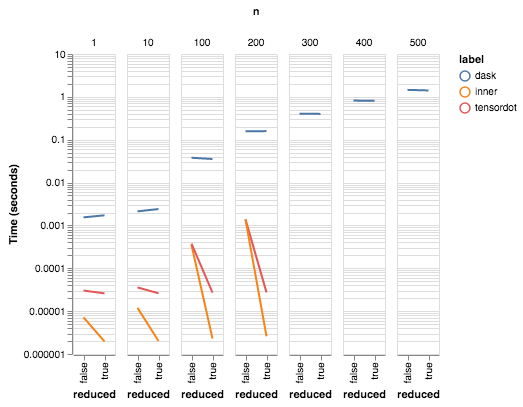
\includegraphics[width=1\textwidth]{benchmarks/visualization.png}
  \caption{The mean execution time of evaluating the expression comparing the original and reduced forms under different shapes and configurations.}
  \label{fig:plot}
\end{figure}

As seen in Figure \ref{fig:plot}, the reduced normal form version is orders of magnitude faster for both the inner and tensordot versions, but not substantially different for the Dask version. 

TODO: Insert table of N, Version, Original (mean), Reduced (mean), Improvement
TODO: Insert appendex section with more detailed benchmarking setup and link to code


\section{Psi Reduction to a Denotational Normal Form (DNF) (TO BE REVISED)}
To $\psi$-R an array expression requires that we:
\begin{enumerate}
    \item We  prove that the shapes of both expressions are equivalent,
    \item We prove all indices based on shapes are equivalent.
\end{enumerate}


We equate the NumPy expressions to MoA expressions. Then we $\psi$-Reduce.
Each time we present a mathematical proof and want to become more mathematical in our explanation we use  {\em MoA} expressions to inform the reader we are doing mathematics without any mention of language. It is important to note that We can translate between the two notations easily  because they are semantically equivalent expressions. We use the {\em syntactic sugar} of Python and NumPy to  converse with the reader. We only change syntax for those interested in the mathematics and want to know more. Moreover, to show long proofs, it is often historic mathematically to use single variable names, and/or complex symbolic expressions.
\subsection{DNF (TO BE REMOVED)}
We will use the same variable names from above except we annotate to indicate dimensionality, e.g. $\vec v$ for a vector and $A^2$ for a matrix, etc.
\begin{eqnarray}
A^3 \equiv \vccc235\reshape(\range30) \\
B^3 \equiv 2+A^3
\end{eqnarray}
$A^3,B^3$ are a and b above.
Let:
\begin{eqnarray}
\vec a \equiv (\vc1\psi( \vc0 \psi (\vccc102 \transpose A^3  ))) \\
\vec b \equiv (\vc0\psi( \vc1 \psi (\vccc102 \transpose B^3  )))\\
%{OP}^2 \equiv \vec a \;\; _{\bf outer}+\;\; \vec b \\
{OP}^2 \equiv \vec a \outerprod\times\vec b\\
%Result \equiv \vec a + _{\bf inner}\times (\vc2 \psi {OP}^2)\\
r \equiv \vec a \innerprod+\times(\vc2 \psi {OP}^2)\\
\end{eqnarray}
To find (1) shape, then (2) components.
\subsection{Get Shape}
\begin{eqnarray}
\shape (\vec a \innerprod+\times \ldots ) \equiv (\minus1 \drop (\shape \vec a) )\cat (1 \drop (\shape (\vc2 \psi {OP}^2))) \\ 
\equiv \minus1 \drop \Theta \cat 1 \drop \Theta
\end{eqnarray}
The shape of a vector is a one element vector, and 1 Drop a one element vector is the empty vector, $\Theta$.
Next, we get components based on shape.

$\forall \vec i s.t. 0  \leq^* \vec i <^* \Theta $ which says that the only valid index vector of an array with empty shape, i.e. a scalar is $\Theta$, the empty vector. 
\begin{eqnarray}
\Theta \psi \vec a \innerprod+\times \vec b \equiv \reduce+ (\vec a \times (\vc2 \psi {OP}^2))
\end{eqnarray}
This is an identity, $\Theta \psi \xi \equiv \xi$ Now get shape of the multiplication.
\begin{eqnarray}
\shape ((\vec a \times (<2> \psi {OP}^2)) \equiv \shape \vec a \equiv  2 \drop (\shape < 1\;0\;2> \transpose A^3 )\equiv 2 \drop \vccc325 \equiv <5>
\end{eqnarray}
$\forall 0 \leq i <5 $
\begin{eqnarray}
\vc i \psi(\vec a \times \vc2\psi {OP}^2) \equiv \vc i \psi \vec a \times \vc i \psi \vc2 \psi {OP}^2 \\
\vc i \psi \vc1 \psi \vc0 \psi \vccc102 \transpose A^3 \equiv \vccc01i \psi \vccc102 A^3\\
\equiv \vccc10i \psi   A^3\\
\vc i \psi  \vc2 {OP}^2 \equiv \vcc2i \psi {OP}^2\\
\equiv \vcc2i \psi {\vec a \outerprod\times \vec b}
\end{eqnarray}
What is shape of $\vec a \outerprod\times \vec b $? 

It is $(2\drop \shape \vccc102\transpose A^3) \cat (2\drop \shape \vccc102 \transpose B^3) \equiv \vcc55$

Therefore, substituting we get:
\[ (\vccc012 \psi A^3) \times \vcc01 \psi B^3\]
This gets the vector we need for the inner product. 

Finally we sum the vector for all i.
\[ \reduce+ (\vcc10\psi A^3) \times(( \vccc102 \psi A^3)\times \vcc01 \psi B^3)\]
\begin{verbatim}
  sum((a[1,0,:] * (a[1,0,2]*b[0,1,:])))
\end{verbatim}

\bibliography{paper}
\bibliographystyle{plain}
\end{document}
